\clearpage
\label{sec:appendix}

\section{Annotator Details}
\label{sec:annotator_details}
All of our datasets relied on two main pools of annotators: domain experts and the authors. The domain expert pool was responsible for:
\begin{enumerate}
    \item The creation of the original set of BFF-Bench questions.
    \item Writing the reference responses for BFF-Bench questions.
    \item Verifying the reference responses for BFF-Bench questions.
    \item Grading the model outputs for the BFF-Bench questions.
    \item Grading the model outputs for the (C)MT-Bench questions.
\end{enumerate}

The authors:
\begin{enumerate}
    \item Edited responses for readability and formatting.
    \item Created and verified responses for the (C)MT-Bench dataset.
    \item Graded the model outputs for the (C)MT-Bench questions.
\end{enumerate}

Our domain expert pool consisted of 9 salaried analysts employed full-time at a financial services company. Each had at least a bachelor's degree in a business or finance discipline. They were based in the United States and Pakistan. They were not compensated beyond their salary for any work performed for the creation of this dataset.

This work did not present any meaningful risk for our annotators. They were volunteers who accepted the work as part of their normal full-time duties. We were in frequent contact to ensure that they understood the goal of the work and its potential impacts. 

\subsection{BFF-Bench}
The annotation process occurred in two main stages: dataset creation and model response grading. To create the dataset we first worked with the annotators to develop a set of initial questions and draft responses. We filtered these responses to find questions that were unambiguous, difficult, and self-contained.

Once we had identified a set of questions to use as the base, we then verified the responses. A subset of the annotators were tasked with reviewing each response for accuracy. If a potential error was found, the annotator would propose a new potential response. This proposed response would then go through the same verification process.

We continued this process until we reached 80 two-turn questions with verified answers.

\subsection{(C)MT-Bench}

(C)MT-Bench was created after our initial analysis into the references in the MT-Bench dataset. We started by manually going through each provided reference in the math and reasoning category and marking them correct or incorrect. We (the authors) then fixed each error by hand, resulting in corrected reference responses.

\subsection{Grading}

The grading process for both datasets occurred within the same user interface. The annotators were given the reference response to the question as a guide and were asked to select whether the model's response was ``Correct'', ``Incorrect'', or ``Not sure''. There was an additional ``Notes'' free response box that they could use to flag any issues that arose. Because the references had been verified, we recommended that the annotators generally err on the side of trusting them. 

The exact guidelines provided to the annotators are provided in the following section (\cref{sec:annotatorguidelines}).

\subsection{Annotator Guidelines}
\label{sec:annotatorguidelines}
The model will attempt to answer the provided question (first text box above the
other two boxes).  A model will generally attempt to fool the judge with
confident wrong answers in cases where it does not know the correct
answer. Annotators will utilize the Reference (bottom left text box), which
contains the answer to the posed question (top text box).

Model Answers should include the relevant facts/formulas needed to answer the
question, with a step-by-step explanation of any mathematical manipulations.

It is important to remember that everything should be graded only with respect
to the reference answer. If you find any errors within the reference, please
mark the error in the notes! However, you should always enter the grade as if
the reference is correct.

A general set of guidelines is:
\begin{enumerate}

        \item If the model’s final answer or recommendation disagrees with the reference, it should be marked “Incorrect”.
        \item If the model agrees with the reference but its intermediate steps disagree, it should also be marked “Incorrect”.
        \item If the model agrees with the reference, all of the intermediate steps agree, and it provides the additional information that is not obviously wrong based on the reference, it should be marked “Correct”
        \item If the model agrees with the reference, all of the intermediate steps agree, but the answer is slightly off due to rounding or performing approximate calculations, it should be marked as “Correct”
        \item If the model agrees with the reference, all of the intermediate steps agree, but it is lacking some amount of information given within the reference, you should make a judgment call as to whether the missing information is crucial to the answer. If you are unsure, lean towards “Correct” or mark it “Unsure”

\end{enumerate}

\subsection{F1 Results}
\label{ref:f1_table}

\begin{table*}[ht!]

    \resizebox{\textwidth}{!}{ %
    \begin{tabular}{l|ccc|ccc|ccc}
    \toprule
    & \multicolumn{9}{c}{\bf Single Grading} \\
    \hline
    & \multicolumn{3}{c|}{Overall} & \multicolumn{3}{c|}{Judge Answered Correctly} & \multicolumn{3}{c}{Judge Answered Incorrectly}\\
& \textit{None} & \textit{Self} & \textit{Human} & \textit{None} & \textit{Self} & \textit{Human} & \textit{None} & \textit{Self} & 
         \textit{Human} \\
\hline
GPT-4o & $0.77_{\pm 0.03 }$ & $0.77_{\pm 0.03 }$ & $\textbf{0.85}_{\pm 0.02 }$ & $0.83_{\pm 0.03 }$ & $0.83_{\pm 0.03 }$ & $0.86_{\pm 0.02 }$ & \R $0.34_{\pm 0.13 }$ & \R $0.30_{\pm 0.13 }$ & $\textbf{0.84}_{\pm 0.12 }$ \\
Llama 3.3 70b & $0.81_{\pm 0.02 }$ & $0.80_{\pm 0.03 }$ & $\textbf{0.91}_{\pm 0.02 }$ & $0.93_{\pm 0.02 }$ & $0.88_{\pm 0.02 }$ & $0.94_{\pm 0.02 }$ & \R $0.39_{\pm 0.07 }$ & \R $0.41_{\pm 0.09 }$ & \R $\textbf{0.76}_{\pm 0.09 }$ \\
Phi 4 & $0.78_{\pm 0.02 }$ & $0.74_{\pm 0.03 }$ & $\textbf{0.88}_{\pm 0.02 }$ & $0.92_{\pm 0.02 }$ & $0.84_{\pm 0.03 }$ & $0.92_{\pm 0.02 }$ & \R $0.32_{\pm 0.07 }$ & \R $0.22_{\pm 0.10 }$ & \R $\textbf{0.65}_{\pm 0.10 }$ \\
Yi 1.5 34B & $0.76_{\pm 0.03 }$ & $0.69_{\pm 0.03 }$ & $\textbf{0.83}_{\pm 0.02 }$ & $0.87_{\pm 0.03 }$ & $0.80_{\pm 0.03 }$ & $0.88_{\pm 0.03 }$ & \R $0.46_{\pm 0.07 }$ & \R $0.37_{\pm 0.08 }$ & \R $\textbf{0.75}_{\pm 0.07 }$ \\
Qwen 2.5 7B & $0.76_{\pm 0.03 }$ & $0.76_{\pm 0.03 }$ & $\textbf{0.85}_{\pm 0.02 }$ & $0.89_{\pm 0.02 }$ & $0.86_{\pm 0.03 }$ & $0.91_{\pm 0.02 }$ & \R $0.45_{\pm 0.07 }$ & \R $0.45_{\pm 0.07 }$ & \R $\textbf{0.70}_{\pm 0.06 }$ \\


\end{tabular}

}
\vspace{1em}
    \resizebox{\textwidth}{!}{ %
    \begin{tabular}{l|ccc|ccc|ccc}
    \toprule
    & \multicolumn{9}{c}{\bf Pairwise Grading} \\
    \hline
    & \multicolumn{3}{c|}{Overall} & \multicolumn{3}{c|}{Judge Answered Correctly} & \multicolumn{3}{c}{Judge Answered Incorrectly}\\
         & \textit{None} & \textit{Self} & \textit{Human} & \textit{None} & \textit{Self} & \textit{Human} & \textit{None} & \textit{Self} & 
         \textit{Human} \\

\hline
GPT-4o & $0.82_{\pm 0.02 }$ & $0.86_{\pm 0.01 }$ & $\textbf{0.95}_{\pm 0.01 }$ & $0.88_{\pm 0.01 }$ & $0.94_{\pm 0.01 }$ & $0.95_{\pm 0.01 }$ & \R $0.62_{\pm 0.06 }$ & \R $0.54_{\pm 0.05 }$ & \R $\textbf{0.90}_{\pm 0.03 }$ \\
Llama 3.3 70b & $0.82_{\pm 0.02 }$ & $0.85_{\pm 0.02 }$ & $\textbf{0.96}_{\pm 0.01 }$ & $0.89_{\pm 0.02 }$ & $0.93_{\pm 0.01 }$ & $\textbf{0.96}_{\pm 0.01 }$ & \R $0.66_{\pm 0.04 }$ & \R $0.65_{\pm 0.04 }$ & $\textbf{0.95}_{\pm 0.02 }$ \\
Phi 4 & $0.75_{\pm 0.02 }$ & $0.80_{\pm 0.02 }$ & $\textbf{0.94}_{\pm 0.01 }$ & $0.88_{\pm 0.02 }$ & $0.95_{\pm 0.01 }$ & $\textbf{0.98}_{\pm 0.01 }$ & \R $0.49_{\pm 0.06 }$ & \R $0.49_{\pm 0.06 }$ & \R $\textbf{0.89}_{\pm 0.03 }$ \\
Yi 1.5 34B & $0.42_{\pm 0.05 }$ & $0.50_{\pm 0.04 }$ & $\textbf{0.81}_{\pm 0.03 }$ & $0.62_{\pm 0.08 }$ & $0.79_{\pm 0.06 }$ & $0.86_{\pm 0.05 }$ & \R $0.27_{\pm 0.06 }$ & \R $0.33_{\pm 0.07 }$ & $\textbf{0.79}_{\pm 0.04 }$ \\
Qwen 2.5 7B & $0.67_{\pm 0.03 }$ & $0.69_{\pm 0.03 }$ & $\textbf{0.85}_{\pm 0.02 }$ & $0.81_{\pm 0.03 }$ & $0.83_{\pm 0.03 }$ & $\textbf{0.89}_{\pm 0.02 }$ & \R $0.47_{\pm 0.05 }$ & \R $0.49_{\pm 0.05 }$ & \R $\textbf{0.78}_{\pm 0.04 }$ \\


\bottomrule
\end{tabular}
}
\caption{Overall results using F1 instead of Cohen's $\kappa$. Cells in \colorbox{red!30}{red} represent cases in which the model is worse when it was wrong as a candidate ($\alpha < 0.05$). Numbers in \textbf{bold} indicate the maximum values on that subset with statistical significance ($\alpha < 0.05$).}
\label{tab:right-wrong-table-f1-v1}
\end{table*}


\subsection{Prompt Sensitivity}
\label{sec:prompt_sensitivity} 

In this section, we compare our main results across two prompts: the slightly modified version of the MT-Bench prompts, and the additional set of prompts we had written from scratch for this analysis. The results are displayed in \cref{tab:right-wrong-table-kappa-v1}. In general, we find the results to be very similar, demonstrating that our analysis is robust to the underlying prompt. 

\begin{table*}[ht!]

    \resizebox{\textwidth}{!}{ %
    \begin{tabular}{l|ccc|ccc|ccc}
    \toprule
    & \multicolumn{9}{c}{\bf Prompt One} \\
    \hline
    & \multicolumn{3}{c|}{Overall} & \multicolumn{3}{c|}{Judge Answered Correctly} & \multicolumn{3}{c}{Judge Answered Incorrectly}\\
& \textit{None} & \textit{Self} & \textit{Human} & \textit{None} & \textit{Self} & \textit{Human} & \textit{None} & \textit{Self} & 
         \textit{Human} \\
\hline
GPT-4o & $0.47_{\pm 0.05 }$ & $0.52_{\pm 0.05 }$ & $\textbf{0.68}_{\pm 0.04 }$ & $0.46_{\pm 0.07 }$ & $0.52_{\pm 0.06 }$ & \R $0.59_{\pm 0.06 }$ & \R $0.16_{\pm 0.14 }$ & \R $0.13_{\pm 0.15 }$ & $\textbf{0.81}_{\pm 0.13 }$ \\
Llama 3.3 70b & $0.42_{\pm 0.05 }$ & $0.53_{\pm 0.05 }$ & $\textbf{0.78}_{\pm 0.04 }$ & $0.62_{\pm 0.09 }$ & $0.54_{\pm 0.08 }$ & $0.74_{\pm 0.07 }$ & \R $0.13_{\pm 0.06 }$ & \R $0.23_{\pm 0.11 }$ & $\textbf{0.69}_{\pm 0.10 }$ \\
Phi 4 & $0.27_{\pm 0.05 }$ & $0.47_{\pm 0.05 }$ & $\textbf{0.72}_{\pm 0.04 }$ & $0.48_{\pm 0.10 }$ & $0.47_{\pm 0.07 }$ & $\textbf{0.67}_{\pm 0.07 }$ & \R $0.03_{\pm 0.05 }$ & \R $0.03_{\pm 0.11 }$ & $\textbf{0.56}_{\pm 0.12 }$ \\
Yi 1.5 34B & $0.38_{\pm 0.06 }$ & $0.37_{\pm 0.05 }$ & $\textbf{0.63}_{\pm 0.05 }$ & $0.23_{\pm 0.11 }$ & $0.29_{\pm 0.07 }$ & \R $0.43_{\pm 0.09 }$ & $0.18_{\pm 0.10 }$ & $0.14_{\pm 0.10 }$ & $\textbf{0.65}_{\pm 0.08 }$ \\
Qwen 2.5 7B & $0.24_{\pm 0.06 }$ & $0.43_{\pm 0.06 }$ & $\textbf{0.63}_{\pm 0.05 }$ & $0.31_{\pm 0.10 }$ & $0.37_{\pm 0.10 }$ & $0.54_{\pm 0.09 }$ & \R $0.08_{\pm 0.07 }$ & $0.21_{\pm 0.10 }$ & $\textbf{0.57}_{\pm 0.08 }$ \\
  


\end{tabular}

}
\vspace{1em}
    \resizebox{\textwidth}{!}{ %
    \begin{tabular}{l|ccc|ccc|ccc}
    \toprule
    & \multicolumn{9}{c}{\bf Prompt Two} \\
    \hline
    & \multicolumn{3}{c|}{Overall} & \multicolumn{3}{c|}{Judge Answered Correctly} & \multicolumn{3}{c}{Judge Answered Incorrectly}\\
         & \textit{None} & \textit{Self} & \textit{Human} & \textit{None} & \textit{Self} & \textit{Human} & \textit{None} & \textit{Self} & 
         \textit{Human} \\

\hline
GPT-4o & $0.47_{\pm 0.06 }$ & $0.53_{\pm 0.06 }$ & $\textbf{0.65}_{\pm 0.05 }$ & $0.47_{\pm 0.07 }$ & $0.53_{\pm 0.07 }$ & $0.57_{\pm 0.07 }$ & \R $0.10_{\pm 0.14 }$ & \R $0.10_{\pm 0.16 }$ & $\textbf{0.67}_{\pm 0.21 }$ \\
Llama 3.3 70b & $0.38_{\pm 0.06 }$ & $0.55_{\pm 0.06 }$ & $\textbf{0.76}_{\pm 0.04 }$ & $0.56_{\pm 0.10 }$ & $0.58_{\pm 0.08 }$ & $0.71_{\pm 0.07 }$ & \R $0.11_{\pm 0.05 }$ & \R $0.21_{\pm 0.11 }$ & $\textbf{0.69}_{\pm 0.09 }$ \\
Phi 4 & $0.33_{\pm 0.06 }$ & $0.55_{\pm 0.05 }$ & $\textbf{0.69}_{\pm 0.05 }$ & $0.45_{\pm 0.09 }$ & $0.61_{\pm 0.07 }$ & $0.71_{\pm 0.07 }$ & \R $0.08_{\pm 0.06 }$ & \R $0.06_{\pm 0.11 }$ & \R $\textbf{0.43}_{\pm 0.11 }$ \\
Yi 1.5 34B & $0.22_{\pm 0.06 }$ & $0.40_{\pm 0.06 }$ & $\textbf{0.63}_{\pm 0.05 }$ & $0.25_{\pm 0.13 }$ & $0.35_{\pm 0.11 }$ & $\textbf{0.62}_{\pm 0.10 }$ & \R $0.05_{\pm 0.06 }$ & $0.17_{\pm 0.09 }$ & $\textbf{0.50}_{\pm 0.08 }$ \\
Qwen 2.5 7B & $0.29_{\pm 0.06 }$ & $0.46_{\pm 0.06 }$ & $\textbf{0.63}_{\pm 0.05 }$ & $0.32_{\pm 0.10 }$ & $0.37_{\pm 0.09 }$ & $0.50_{\pm 0.09 }$ & \R $0.10_{\pm 0.08 }$ & $0.23_{\pm 0.11 }$ & $\textbf{0.59}_{\pm 0.09 }$ \\

\bottomrule
\end{tabular}
}
\caption{Performance comparison on single grading using the two sets of prompts. Cells in \colorbox{red!30}{red} represent cases in which the model is worse when it was wrong as a candidate ($\alpha < 0.05$). Numbers in \textbf{bold} indicate the maximum values on that subset with statistical significance ($\alpha < 0.05$).}
\label{tab:right-wrong-table-kappa-v1}
\end{table*}


\section{Judgment Prompts}
\label{sec:judgeprompts}
\subsection{Single, Reference, Turn One}
\noindent\textbf{System Prompt:}

\noindent You are a helpful assistant.

\noindent\textbf{Prompt Template:}
\begin{lstlisting}

[Instruction]
Please act as an impartial judge and evaluate the correctness of the response provided by an AI assistant to the user question. You will be given a reference correct answer and the assistant's answer. The reference answer is always correct. Begin you evaluation by comparing the assistant's answer to the correct answer. Identify any mistakes. Be as objective as possible. After providing your explanation, you must rule whether the response is correct or incorrect. Output your final verdict by strictly following this format: "[[Correct]]" if the answer is correct and "[[Incorrect]]" is the answer is incorrect.

[Question]
{question}

[The Start of Reference Answer]
{ref_answer_1}
[The End of Reference Answer]

[The Start of Assistant's Answer]
{answer}
[The End of Assistant's Answer]

\end{lstlisting}

\subsection{Single, Reference, Turn Two}
\noindent\textbf{System Prompt:}

\noindent Please act as an impartial judge and evaluate the correctness of the response provided by an AI assistant to the user question. You will be given a reference correct answer and the assistant's answer. The reference answer is always correct. You should only focus on the assitants answer to the second question. Begin you evaluation by comparing the assistant's answer to the correct answer. Identify any mistakes. Be as objective as possible. After providing your explanation, you must rule whether the response is correct or incorrect. Output your final verdict by strictly following this format: "[[Correct]]" if the answer is correct and "[[Incorrect]]" is the answer is incorrect.

\noindent \textbf{Prompt Template:}
\begin{lstlisting}

<|The Start of Reference Answer|>

### User:
{question_1}

### Reference answer:
{ref_answer_1}

### User:
{question_2}

### Reference answer:
{ref_answer_2}

<|The End of Reference Answer|>


<|The Start of Assistant A's Conversation with User|>

### User:
{question_1}

### Assistant A:
{answer_1}

### User:
{question_2}

### Assistant A:
{answer_2}

<|The End of Assistant A's Conversation with User|>
\end{lstlisting}



\subsection{Single, No Reference, Turn One}
\noindent\textbf{System Prompt:}

\noindent You are a helpful assistant.

\noindent\textbf{Prompt Template:}
\begin{lstlisting}

[Instruction]
Please act as an impartial judge and evaluate the correctness of the response provided by an AI assistant to the user question. You will only be given the assistant's answer. Identify any mistakes. Be as objective as possible. After providing your analysis, you must rule whether the response is correct or incorrect. Output your final verdict by strictly following this format: "[[Correct]]" if the answer is correct and "[[Incorrect]]" is the answer is incorrect.

[Question]
{question}

[The Start of Assistant's Answer]
{answer}
[The End of Assistant's Answer]

\end{lstlisting}

\subsection{Single, No Reference, Turn Two}
\noindent\textbf{System Prompt:}

\noindent Please act as an impartial judge and evaluate the correctness of the responses provided by two AI assistants to the user questions. You should choose the assistant that gives the more correct response. Your evaluation should only consider correctness. You should focus on who provides a more correct answer to the second user question. Begin your evaluation by comparing the responses of the two assistants and provide a short explanation. Avoid any position biases and ensure that the order in which the responses were presented does not influence your decision. Do not allow the length of the responses to influence your evaluation. Do not favor certain names of the assistants. Be as objective as possible. After providing your explanation, output your final verdict by strictly following this format: "[[A]]" if assistant A is more correct, and "[[B]]" if assistant B is more correct.

\noindent\textbf{Prompt Template:}
\begin{lstlisting}

<|The Start of Assistant A's Conversation with User|>

### User:
{question_1}

### Assistant A:
{answer_a_1}

### User:
{question_2}

### Assistant A:
{answer_a_2}

<|The End of Assistant A's Conversation with User|>


<|The Start of Assistant B's Conversation with User|>

### User:
{question_1}

### Assistant B:
{answer_b_1}

### User:
{question_2}

### Assistant B:
{answer_b_2}

<|The End of Assistant B's Conversation with User|>
\end{lstlisting}








\subsection{Pairwise, Reference, Turn One}

\noindent\textbf{System Prompt:}

\noindent Please act as an impartial judge and evaluate the correctness of the responses provided by two AI assistants to the user question displayed below. Your evaluation should consider only correctness. You will be given a reference answer, assistant A's answer, and assistant B's answer. The reference answer is always correct. Your job is to evaluate which assistant's answer is more correct. Begin your evaluation by comparing both assistants' answers with the reference answer. Identify any mistakes. Avoid any position biases and ensure that the order in which the responses were presented does not influence your decision. Do not allow the length of the responses to influence your evaluation. Do not favor certain names of the assistants. Be as objective as possible. After providing your explanation, output your final verdict by strictly following this format: "[[A]]" if assistant A is more correct, and "[[B]]" if assistant B is more correct.

\noindent\textbf{Prompt Template:}
\begin{lstlisting}

[User Question]
{question}

[The Start of Reference Answer]
{ref_answer_1}
[The End of Reference Answer]

[The Start of Assistant A's Answer]
{answer_a}
[The End of Assistant A's Answer]

[The Start of Assistant B's Answer]
{answer_b}
[The End of Assistant B's Answer]
\end{lstlisting}


\subsection{Pairwise, Reference, Turn Two}
\noindent\textbf{System Prompt:}

\noindent Please act as an impartial judge and evaluate the quality of the responses provided by two AI assistants to the user questions. Your evaluation should consider only correctness. You will be given reference answers, the assistant A's answers, the assistant B's answers. The reference answer is always correct. Your job is to determine which assistant provides a more correct answer to the second user question. Begin your evaluation by comparing both assistants' answers with the reference answers. Identify any mistakes. Avoid any position biases and ensure that the order in which the responses were presented does not influence your decision. Do not allow the length of the responses to influence your evaluation. Do not favor certain names of the assistants. Be as objective as possible. After providing your explanation, output your final verdict by strictly following this format: "[[A]]" if assistant A is more correct, and "[[B]]" if assistant B is more correct.

\noindent\textbf{Prompt Template:}
\begin{lstlisting}

<|The Start of Reference Answer|>

### User:
{question_1}

### Reference answer:
{ref_answer_1}

### User:
{question_2}

### Reference answer:
{ref_answer_2}

<|The End of Reference Answer|>


<|The Start of Assistant A's Conversation with User|>

### User:
{question_1}

### Assistant A:
{answer_a_1}

### User:
{question_2}

### Assistant A:
{answer_a_2}

<|The End of Assistant A's Conversation with User|>


<|The Start of Assistant B's Conversation with User|>

### User:
{question_1}

### Assistant B:
{answer_b_1}

### User:
{question_2}

### Assistant B:
{answer_b_2}

<|The End of Assistant B's Conversation with User|>
\end{lstlisting}


\subsection{Pairwise, No Reference, Turn One}
\noindent\textbf{System Prompt:}

\noindent Please act as an impartial judge and evaluate the correctness of the responses provided by two AI assistants to the user question displayed below. You should choose the assistant that gives the more correct response. Your evaluation should only consider correctness. Begin your evaluation by comparing the two responses and provide a short explanation. Avoid any position biases and ensure that the order in which the responses were presented does not influence your decision. Do not allow the length of the responses to influence your evaluation. Do not favor certain names of the assistants. Be as objective as possible. After providing your explanation, output your final verdict by strictly following this format: "[[A]]" if assistant A is more correct, and "[[B]]" if assistant B is more correct.

\noindent\textbf{Prompt Template:}
\noindent\begin{lstlisting}

[User Question]
{question}

[The Start of Assistant A's Answer]
{answer_a}
[The End of Assistant A's Answer]

[The Start of Assistant B's Answer]
{answer_b}
[The End of Assistant B's Answer]
\end{lstlisting}

\subsection{Pairwise, No Reference, Turn Two }
\noindent\textbf{System Prompt:}

\noindent Please act as an impartial judge and evaluate the correctness of the response provided by an AI assistant to the user question. You will only be given the assistant's answer. You should only focus on the assitant's answer to the second question. Identify any mistakes. Be as objective as possible. After providing your analysis, you must rule whether the response is correct or incorrect. Output your final verdict by strictly following this format: "[[Correct]]" if the answer is correct and "[[Incorrect]]" is the answer is incorrect.

\noindent\textbf{Prompt Template:}
\begin{lstlisting}

<|The Start of Assistant A's Conversation with User|>

### User:
{question_1}

### Assistant A:
{answer_1}

### User:
{question_2}

### Assistant A:
{answer_2}

<|The End of Assistant A's Conversation with User|>
\end{lstlisting}


\section{(C)MT-Bench Examples}
\label{sec:cmt_examples}

In this section, we provide an example of an error from MT-Bench. 


\begin{figure}[ht!]
\small
\begin{tcolorbox}[
        enhanced jigsaw, 
        colback=gray!5!white, 
        colframe=gray!90!black, 
        boxrule=1pt, 
        arc=5pt, 
        sharp corners=downhill, 
        left=0pt, right=0pt, top=0pt, bottom=0pt,
        title=MT-Bench Question
    ]
  The vertices of a triangle are at points (0, 0), (-1, 1), and (3, 3). What is the area of the triangle?
\end{tcolorbox}

 \begin{tcolorbox}[
        enhanced jigsaw, 
        colback=providedbg, 
        colframe=providedborder, 
        boxrule=1pt, 
        arc=5pt, 
        sharp corners=downhill, 
        left=0pt, right=0pt, top=0pt, bottom=0pt,
        title=MT-Bench Reference
    ]
To find the area of the triangle, we can use the formula for the area of a triangle with coordinates A(x1, y1), B(x2, y2), and C(x3, y3):

\vspace{0.25em}


Area = (1/2) * |(x1(y2 - y3) + x2(y3 - y1) + x3(y1 - y2))|

\vspace{0.25em}


In this case, the coordinates are A(0, 0), B(-1, 1), and C(3, 3). Plugging these values into the formula, we get:

\vspace{0.25em}


Area = (1/2) * |(0(1 - 3) + (-1)(3 - 0) + 3(0 - 1))|

Area = (1/2) * |(-0 + \hl{{\bf 3}} - 3)|

Area = (1/2) * |0|

Area = 0

\vspace{0.25em}


The area of the triangle is 0. This means that the three points are collinear, and there is no triangle formed by these points.
\end{tcolorbox}

\caption{Example of an incorrect reference included in MT-Bench (\hl{\bf 3} should be $-3$). The correct answer is that the area of the triangle is 3.}
\label{fig:mt-bench-wrong}
\end{figure}




\section{Confidence Intervals on Agreement}
\label{sec:confidenceintervals}

To evaluate the agreement between the judges and the human annotators' consensus, we use the Cohen's $\kappa$ metric \cite{CohenKappa}. This is an agreement measure for categorical data labeled by two raters that accounts for the chance of random agreement. It is defined as:
\begin{equation}
\kappa = 1 - \frac{1 - p_o}{1 - p_e},
\end{equation}
where $p_o$ is the observed agreement and $p_e$ is the expected chance agreement. $\kappa$ is bounded between -1 and 1, with -1 corresponding to no agreement, 0 corresponding to random agreement and 1 corresponding to total agreement. 

For simplicity, we used a boostrap to compute confidence intervals for each of our metrics. Although the intervals that we compute are non-symmetric, we convert them into symmetric intervals for a more compact display in tables. To do so, we select whichever bound leads to the widest interval.

\begin{figure*}[ht]
    \centering
    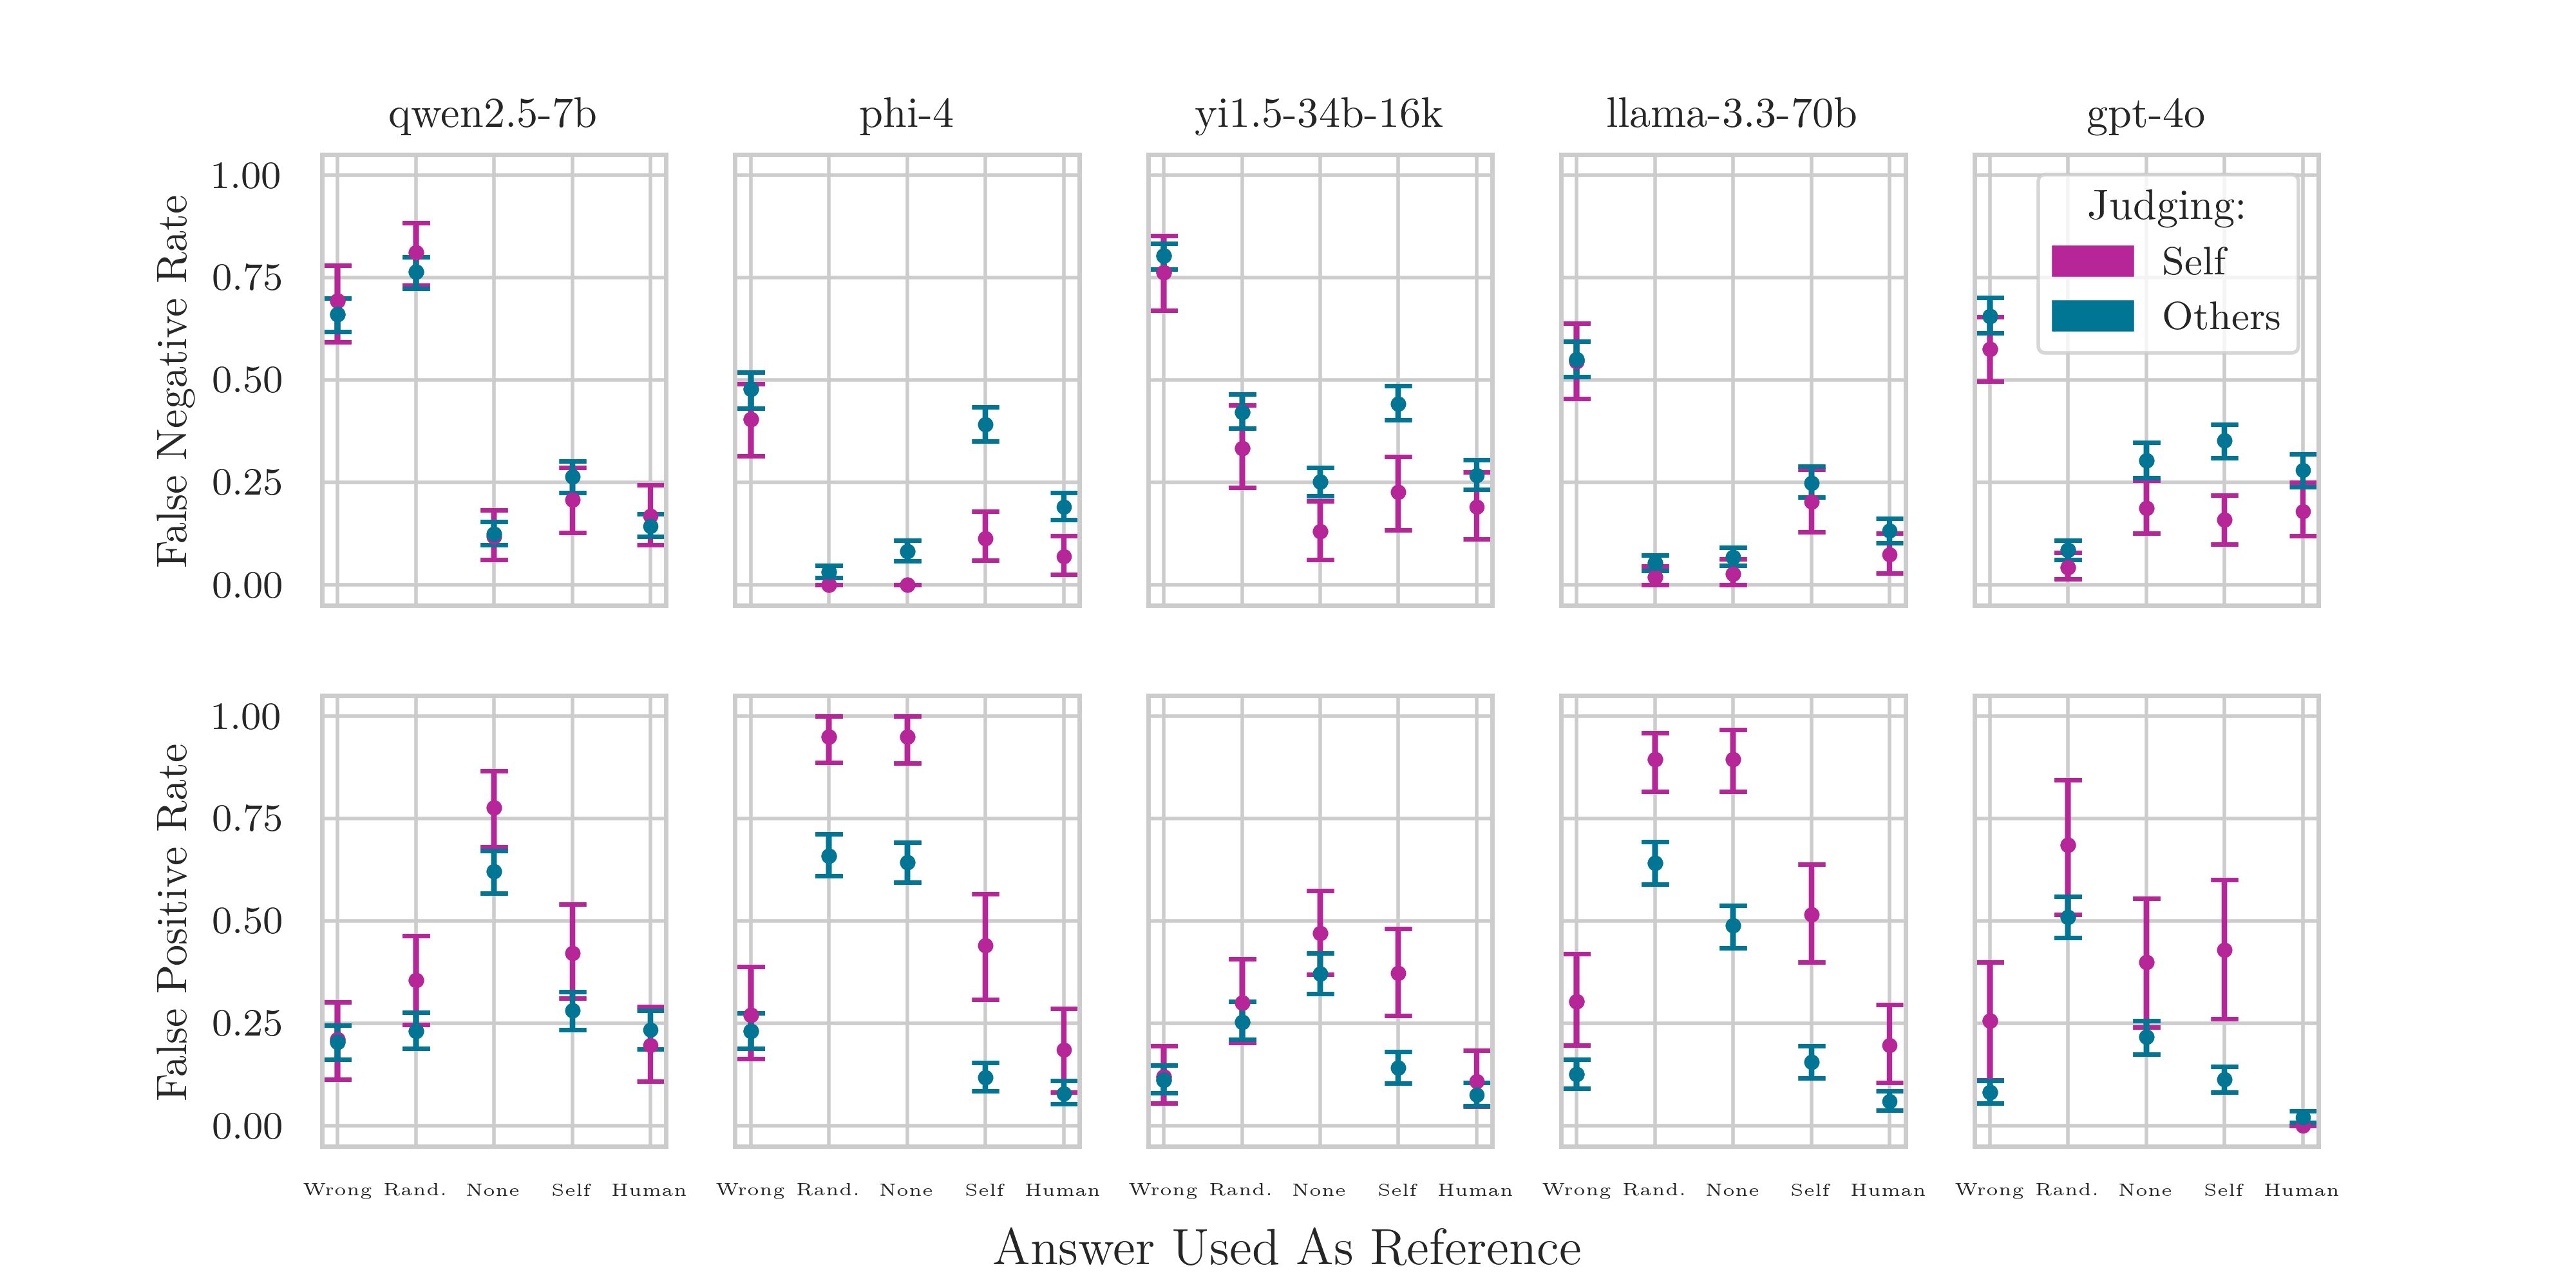
\includegraphics[width=\linewidth]{figures/affinity_bias_all.png}
    \caption{The full graph displaying the error rates for different LLM Judges and different reference types. The same trend displayed in \cref{fig:affinity_bias} holds for each model. Rand. refers to the Random reference type.}
    \label{fig:affinity_per_judge_all}
\end{figure*}


\section{BFF-Bench Examples}
\label{sec:bff-bench-examples}
\begin{figure}[ht!]

\centering
\small

\begin{tcolorbox}[
    boxsep=1pt,
    left=2pt,right=2pt,top=2pt,bottom=2pt,
    colback=blue!5!white,
    colframe=blue!40!black,
    before skip=2pt,
    after skip=2pt,
    sharp corners
]
\textbf{Question (Turn One):}
What is the IFRS 16 treatment of short term or low value leased assets? 
What are the restrictions?
\end{tcolorbox}

\begin{tcolorbox}[
    boxsep=1pt,
    left=2pt,right=2pt,top=2pt,bottom=2pt,
    colback=green!2!white,
    colframe=green!25!black,
    before skip=1pt,
    after skip=3pt,
    sharp corners
]
\small
\textbf{Gold Response:}
IFRS 16 Leases permit a simplified treatment for assets with a lease period of 12 months or less, or of low value. Although the standard does not give a numerical definition of 'low value' it does give examples of the types of assets that may be included, and this includes telephones. The simplified treatment allows the lease payments to be charged as an expense over the lease period, applying the accruals concept.

IFRS 16 Leases does not specify a particular monetary amount below which an asset would be considered 'low value', although the basis for conclusion indicates a value of \$5,000 as a guide. The standard also gives the following examples of low-value assets:

- tablets

- small personal computers

- telephones

- small items of furniture.

The assessment of whether an asset qualifies as having a 'low value' must be made based on its value when new. Therefore, a car would not qualify as a low-value asset, even if it was very old at the commencement of the lease.
\end{tcolorbox}

\begin{tcolorbox}[
    boxsep=1pt,
    left=2pt,right=2pt,top=2pt,bottom=2pt,
    colback=blue!5!white,
    colframe=blue!40!black,
    before skip=3pt,
    after skip=1pt,
    sharp corners
]
\small
\textbf{Question (Turn Two):}
On April 1st 2023, Abigail acquired telephones for her salesforce under a 
two-year lease agreement. The terms of the lease require an initial payment 
of \$3,000, followed by a payment of \$9,000 on March 31st 2024 and an 
additional \$9,000 on March 31st 2025. Show the impact of this lease 
arrangement on Abigail's financial statements for the year ended 
31 December 2023 under IFRS 16?
\end{tcolorbox}

\begin{tcolorbox}[
    boxsep=1pt,
    left=2pt,right=2pt,top=2pt,bottom=2pt,
    colback=green!2!white,
    colframe=green!25!black,
    before skip=1pt,
    after skip=2pt,
    sharp corners=downhill,
]
\small
\textbf{Gold Response:}
\[
\begin{aligned}
\text{Annual lease rental expense} &= \frac{\text{Total rentals payable}}{\text{Total lease period}} = \frac{\$3,000 + \$9,000 + \$9,000}{2\text{ years}} \\[6pt]
&= \$10,500\text{ per annum} \\[8pt]
\text{Expense to 31 December 2023} &= \$10,500 \times \frac{9}{12} = \$7,875 \\[8pt]
\text{Accrued expense} &= \$7,875 - \$3,000 = \$4,875
\end{aligned}
\]

The expense in this period of \$7,875 is not the same as the payment of \$3,000, so we need to accrue an additional expense of \$4,875.
\end{tcolorbox}


\caption{Untruncated example from BFF-Bench.}
\label{fig:bffbench-sample-full}
\end{figure}

\begin{figure}[ht!]
\centering
\small

\begin{tcolorbox}[
    boxsep=1pt, left=2pt,right=2pt,top=2pt,bottom=2pt,
    colback=blue!5!white, colframe=blue!40!black,
    before skip=2pt, after skip=2pt, sharp corners
]
\textbf{Question (Turn One):}  
What is the loan-to-value (LTV) ratio for Class A of the following structured finance securities? Assume a loan amount of \$407 million and an as-is appraised value of the underlying securities of \$550,750,000. Also, keep in mind that the total required credit risk retention percentage (RR interest) for this transaction is 5.00\%.


\begin{tabular}{lc}

CLASS & PRELIMINARY AMOUNT \$) \\
A & 183,160,000 \\
B & 59,185,000 \\
C & 43,890,000 \\
D & 58,178,000 \\
E & 42,237,000 \\
RR interest & 20,350,000 \\

\end{tabular}
\end{tcolorbox}

\begin{tcolorbox}[
    boxsep=1pt, left=2pt,right=2pt,top=2pt,bottom=2pt,
    colback=green!2!white, colframe=green!25!black,
    before skip=1pt, after skip=3pt, sharp corners
]
\small
\textbf{Gold Response:}
1.) The total loan amount is \$407 million.

2.) The as-is appraised value of the underlying collateral is \$550,744,248.99.

3.) The required RR interest (credit risk retention) is 5.00\% of the total loan amount, or 20,350,000. 



The RR interest represents the portion of the loan that the sponsor retains in order to share the risk. This amount is subtracted from the appraised value since it's not part of the bondholder allocation.
\[
\$550,744,248 - \$20,350,000 =  \$530,394,248.99        
\]
Next, divide the Class A balance by \$530,394,248.99: 
\[
\$183,160,000 / \$530,394,248.99 = 0.3453
\]
The LTV of Class A is approximately 34.53\%, or 35\% when rounded to the nearest percent.
\end{tcolorbox}

\begin{tcolorbox}[
    boxsep=1pt, left=2pt,right=2pt,top=2pt,bottom=2pt,
    colback=blue!5!white, colframe=blue!40!black,
    before skip=3pt, after skip=1pt, sharp corners
]
\small
\textbf{Question (Turn Two):}  
If the RR interest balance of \$20,350,000 is instead allocated to Class E, how does this affect the loan-to-value (LTV) ratio for Class A?
\end{tcolorbox}

\begin{tcolorbox}[
    boxsep=1pt, left=2pt,right=2pt,top=2pt,bottom=2pt,
    colback=green!2!white, colframe=green!25!black,
    before skip=1pt, after skip=2pt, sharp corners=downhill,
]
\small
\textbf{Gold Response:}
In this scenario, the new balance of Class E is the original Class E balance of  \$42,237,000 plus the previous RR balance of \$20,350,000, or \$62,587,000.

Since the RR class is no longer a factor, the Appraisal value is \$550,750,000. Therefore, the Class A LTV is simply the Class A balance divided by the Appraisal value, or 
\[
183,160,000 / \$550,750,000 = ~33.24\%,
\]
or 33\% if rounded to the nearest percent. 

\end{tcolorbox}

\caption{Untruncated example from BFF-Bench.}
\label{fig:bffbench-sample-full-2}
\end{figure}



\section{Baselines}
\label{sec:baselines}

\begin{table*}[ht]
\centering
\begin{tabular}{lc}
\toprule
 & Cohen's $\kappa$ \\
 \midrule
\textit{Reward Models} & \\
\texttt{INF-ORM-Llama3.1-70B} & $0.44_{\pm 0.07 }$ \\
\texttt{Llama-3.1-Nemotron-70B-Reward} & $0.37_{\pm 0.07 }$ \\
\texttt{LDL-Reward-Gemma-2-27B-v0.1} & $0.31_{\pm 0.08 }$ \\
\texttt{Skywork-Reward-Gemma-2-27B-v0.2} & $0.30_{\pm 0.07 }$ \\
\texttt{QRM-Gemma-2-27B} & $0.24_{\pm 0.08 }$ \\
\midrule
\textit{Embedding Models} & \\
\texttt{Linq-AI-Research/Linq-Embed-Mistral} & $0.35_{\pm 0.08 }$ \\
\texttt{NovaSearch/jasper\_en\_vision\_language\_v1} & $0.34_{\pm 0.07 }$ \\
\texttt{Salesforce/SFR-Embedding-Mistral} & $0.25_{\pm 0.08 }$ \\
\texttt{Alibaba-NLP/gte-Qwen2-7B-instruct} & $0.21_{\pm 0.08 }$ \\
\texttt{intfloat/e5-mistral-7b-instruct} & $0.18_{\pm 0.08 }$ \\
\midrule
\textit{{Lexical}} & \\
METEOR & $0.28_{\pm 0.08 }$ \\
ROUGE & $0.26_{\pm 0.08 }$ \\
BLEU & $0.15_{\pm 0.08 }$ \\
\bottomrule
\label{tab:baseline_perf}
\end{tabular}

\caption{Full results table for all baselines on the pairwise grading task.}
\end{table*}

\subsection{Reward Models}
We selected the top five performing models on RewardBench \cite{RewardBench}: 

\begin{itemize}
    \item \url{INF-ORM-Llama3.1-70B}, \citet{INF-ORM-Llama3.1-70B}
    \item \url{LDL-Reward-Gemma-2-27B-v0.1}, \citet{}{LDL-Reward-Gemma-2-27B-v0.1}
    \item \url{QRM-Gemma-2-27B}, \citet{dorka2024quantile}
    \item \url{Skywork-Reward-Gemma-2-27B-v0.2}, \citet{liu2024skywork}
    \item \url{Llama-3.1-Nemotron-70B-Reward}, \citet{wang2024helpsteer2preferencecomplementingratingspreferences,wang2024helpsteer2}
\end{itemize}

To run the pairwise evaluation, we extracted the reward for each of the potential responses and ruled the ``more correct'' one to be the one with the higher reward.

\subsection{Reference-Based Lexical Overlap Classifiers}
We implement a series of reference based classifiers. For each of these classifiers, we compute a similarity score between the human-written reference and each of the two provided responses. We then rule the response with the higher similarity with the human-written reference to be ``Correct''.

We used the \texttt{evaluate} library (0.4.3) \cite{evaluate} to compute ROUGE, BLEU and METEOR scores. We used the default settings for each metric. 

\subsection{Embedding Models}

We selected the following five Embedding Models using \cite{mteb}:
\begin{itemize}
    \item \url{Linq-AI-Research/Linq-Embed-Mistral}, \citet{linq}
    \item \url{NovaSearch/jasper_en_vision_language_v1}, \citet{zhang2024jasper}
    \item \url{Salesforce/SFR-Embedding-Mistral}, \citet{SFRAIResearch2024}
    \item \url{Alibaba-NLP/gte-Qwen2-7B-instruct}, \citet{li2023towards}
    \item \url{intfloat/e5-mistral-7b-instruct}, \citet{wang2023improving,wang2022text}
\end{itemize}
For the embedding metrics, we computed the cosine similarity between the embeddings of the human-written reference and the two responses.



\section{Judge Refusal}
\label{sec:judge-refusal}

The following example is \texttt{GPT-4o} grading a response from \texttt{Phi-4} using a wrong reference which inverts the definition of annuities and IRAs. The text generated by \texttt{GPT-4o} notes the inconsistencies between the reference and the response, but overrules the reference and still marks the response as correct. We observed this behavior multiple times, only with \texttt{GPT-4o}.
\\\\
\noindent\textbf{Judgment:}

The assistant's answer provides a breakdown of the differences between annuities and IRAs, similar to the reference answer. Let's compare the key elements:

1. \textit{Annuity}:
   - The assistant correctly identifies annuities as financial products designed to provide a steady income stream, and they can be immediate or deferred. It mentions different types of annuities (fixed, variable, indexed) and notes the tax-deferred nature of annuities and the penalties for early withdrawal.
   - The reference answer describes annuities as investment accounts for holding financial assets, emphasizing accumulating contributions and interest until retirement age, and mentions custodial fees and mutual funds' expense ratios.
   - There is a discrepancy in the definition: the reference answer incorrectly describes annuities as accounts for holding investments, which aligns more with the description of IRAs.

2. \textit{IRA}:
   - The assistant correctly describes IRAs as tax-advantaged savings accounts with different types (Traditional and Roth) and their unique tax implications. It covers tax treatment, access to funds, and ownership.
   - The reference answer incorrectly labels IRAs as insurance products, which is inaccurate. It also incorrectly suggests IRAs do not have contribution limits, which is a mistake.

3. \textit{Key Differences}:
   - The assistant highlights investment control, flexibility, tax treatment, and income stream as key differences, which are generally accurate and align with the correct understanding of annuities and IRAs.

Overall, the reference answer contains significant inaccuracies regarding the fundamental nature of annuities and IRAs. In contrast, the assistant's answer provides a more accurate description and comparison of these financial products.

[[Correct]]



